\section{Userinterface}

	Für einen Erstentwurf des Userinterface hat das Team ein Wireframe-Brainstorming durchgeführt.
	Dazu hat jedes Teammitglied Wireframes und Workflows entworfen.

	\begin{figure}[H]
		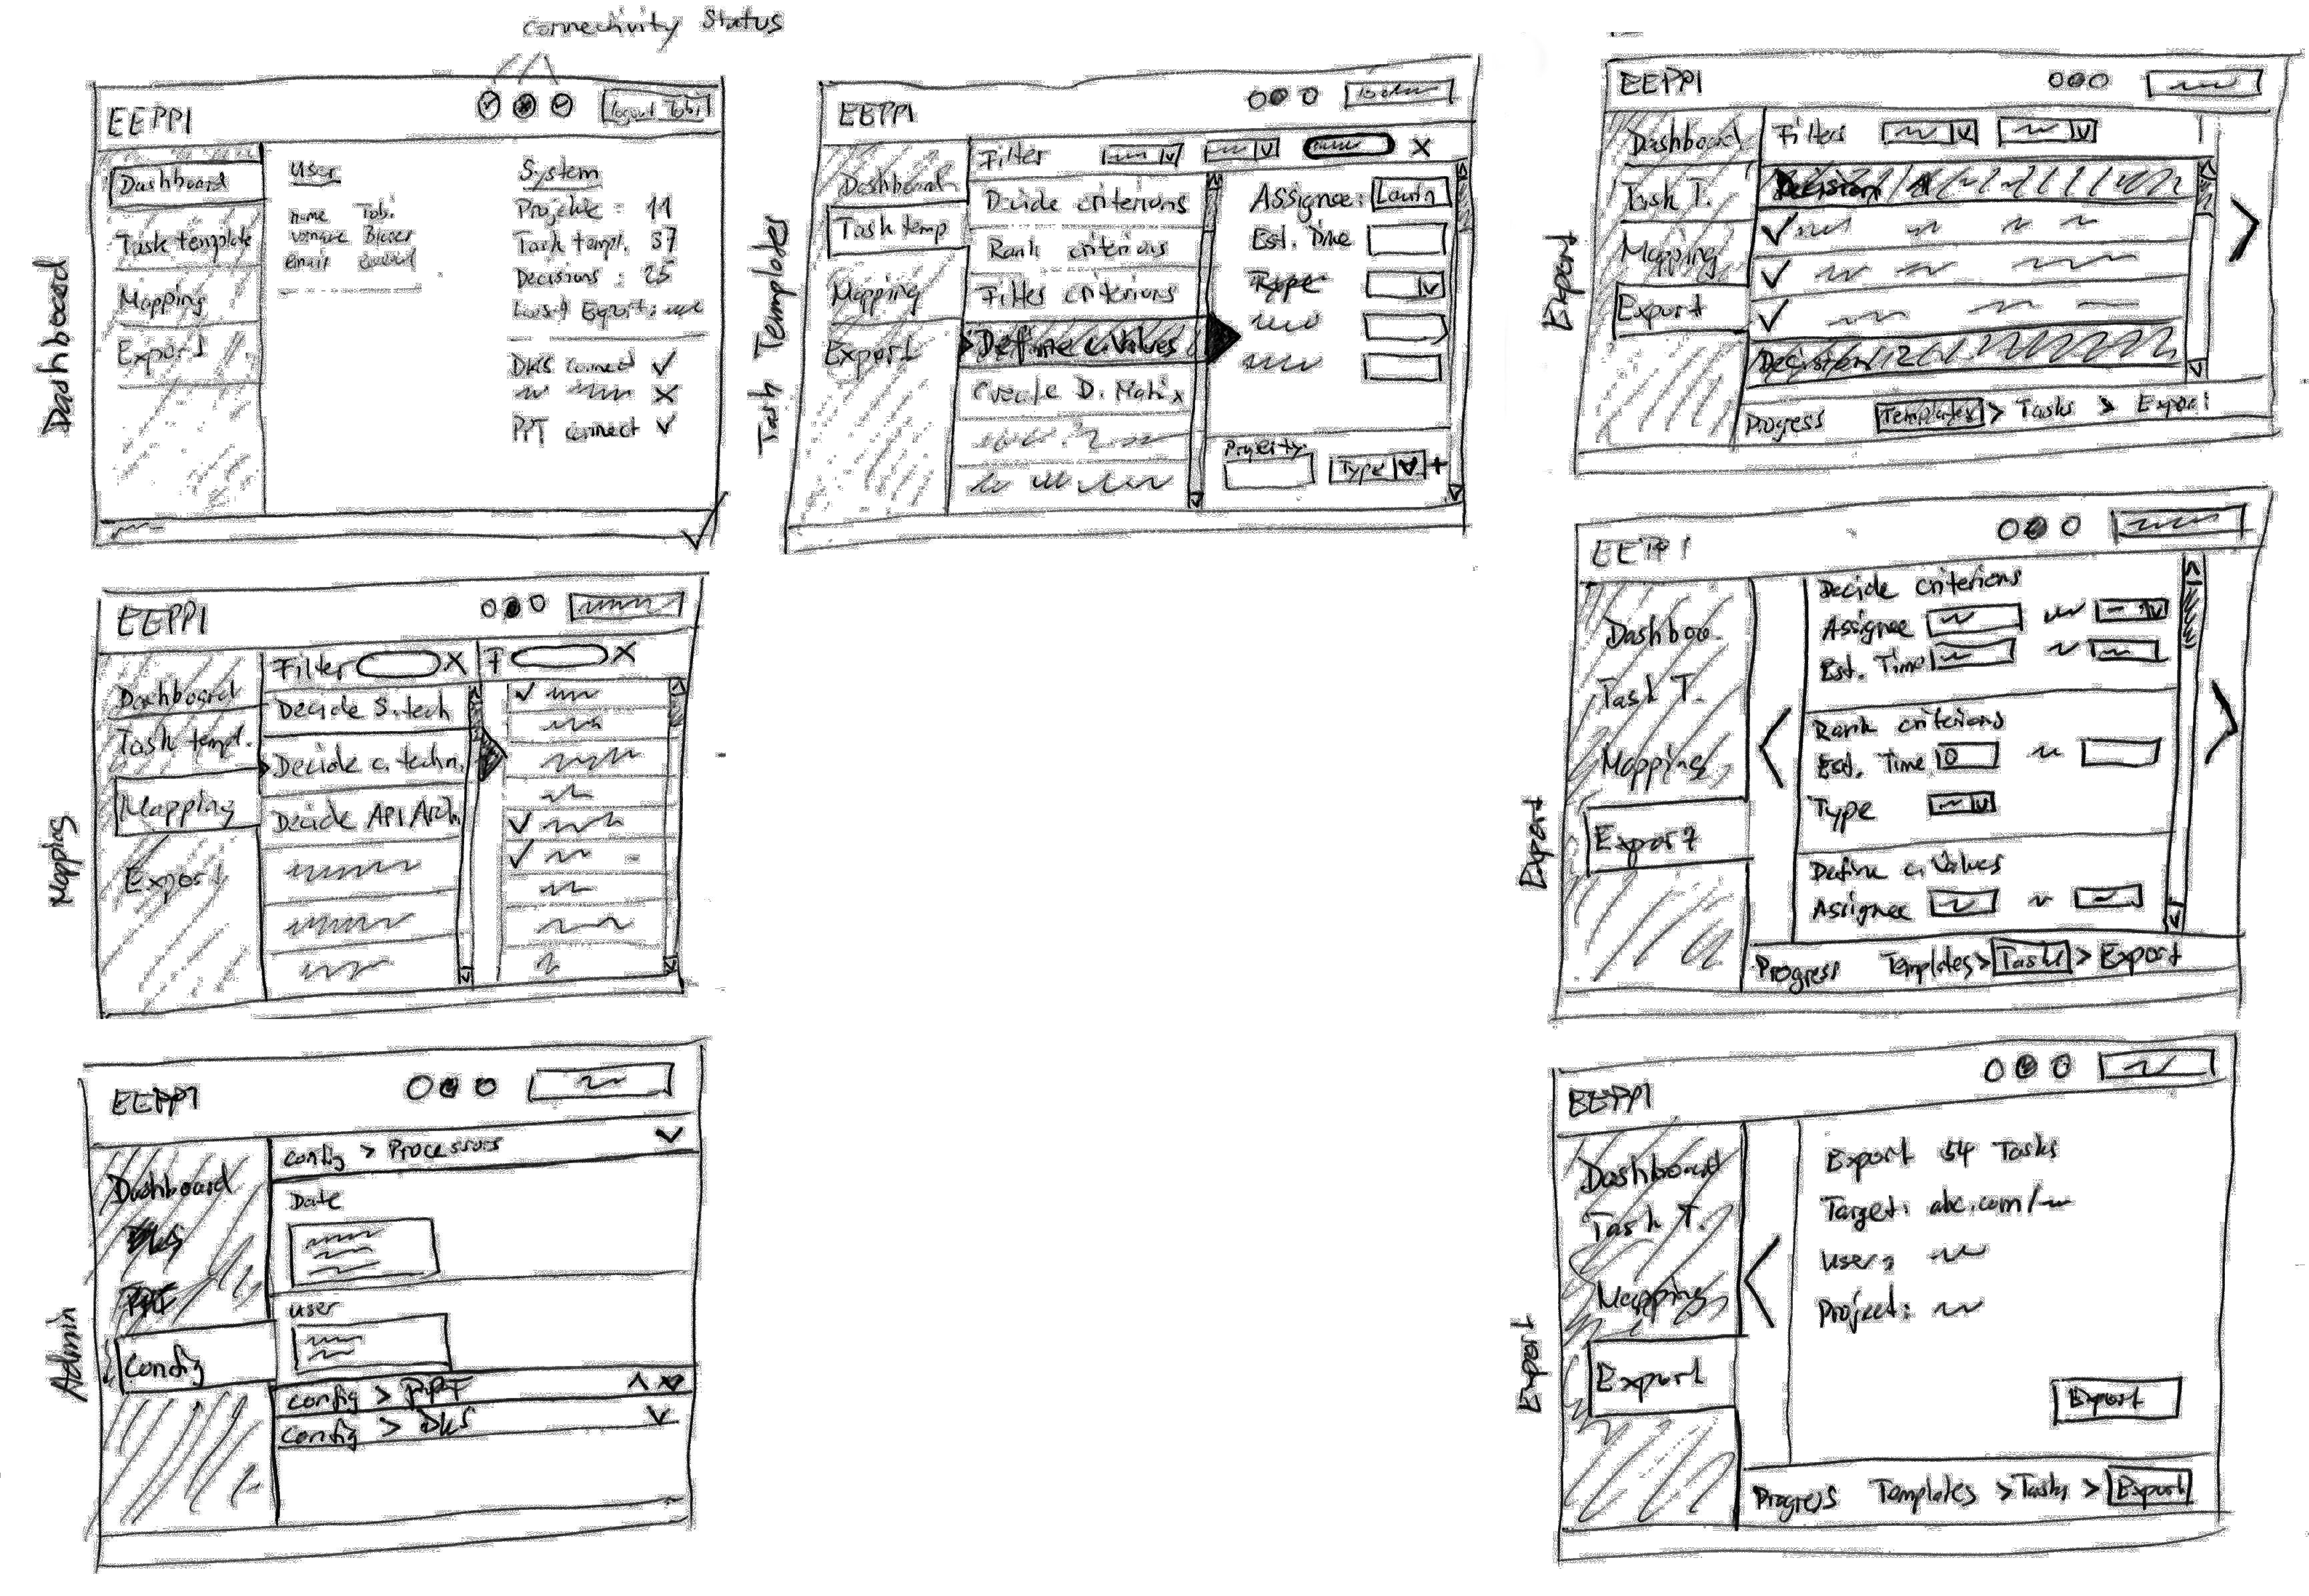
\includegraphics[width=\linewidth]{interfacesAndProtocols/media/img/wireframesTobias1.jpg}
		\centering
		\caption{Wireframes Tobias}
		\label{fig:wireframesTobias1}
	\end{figure}
	
	\begin{figure}[H]
		\begin{minipage}[b]{0.5\linewidth}
			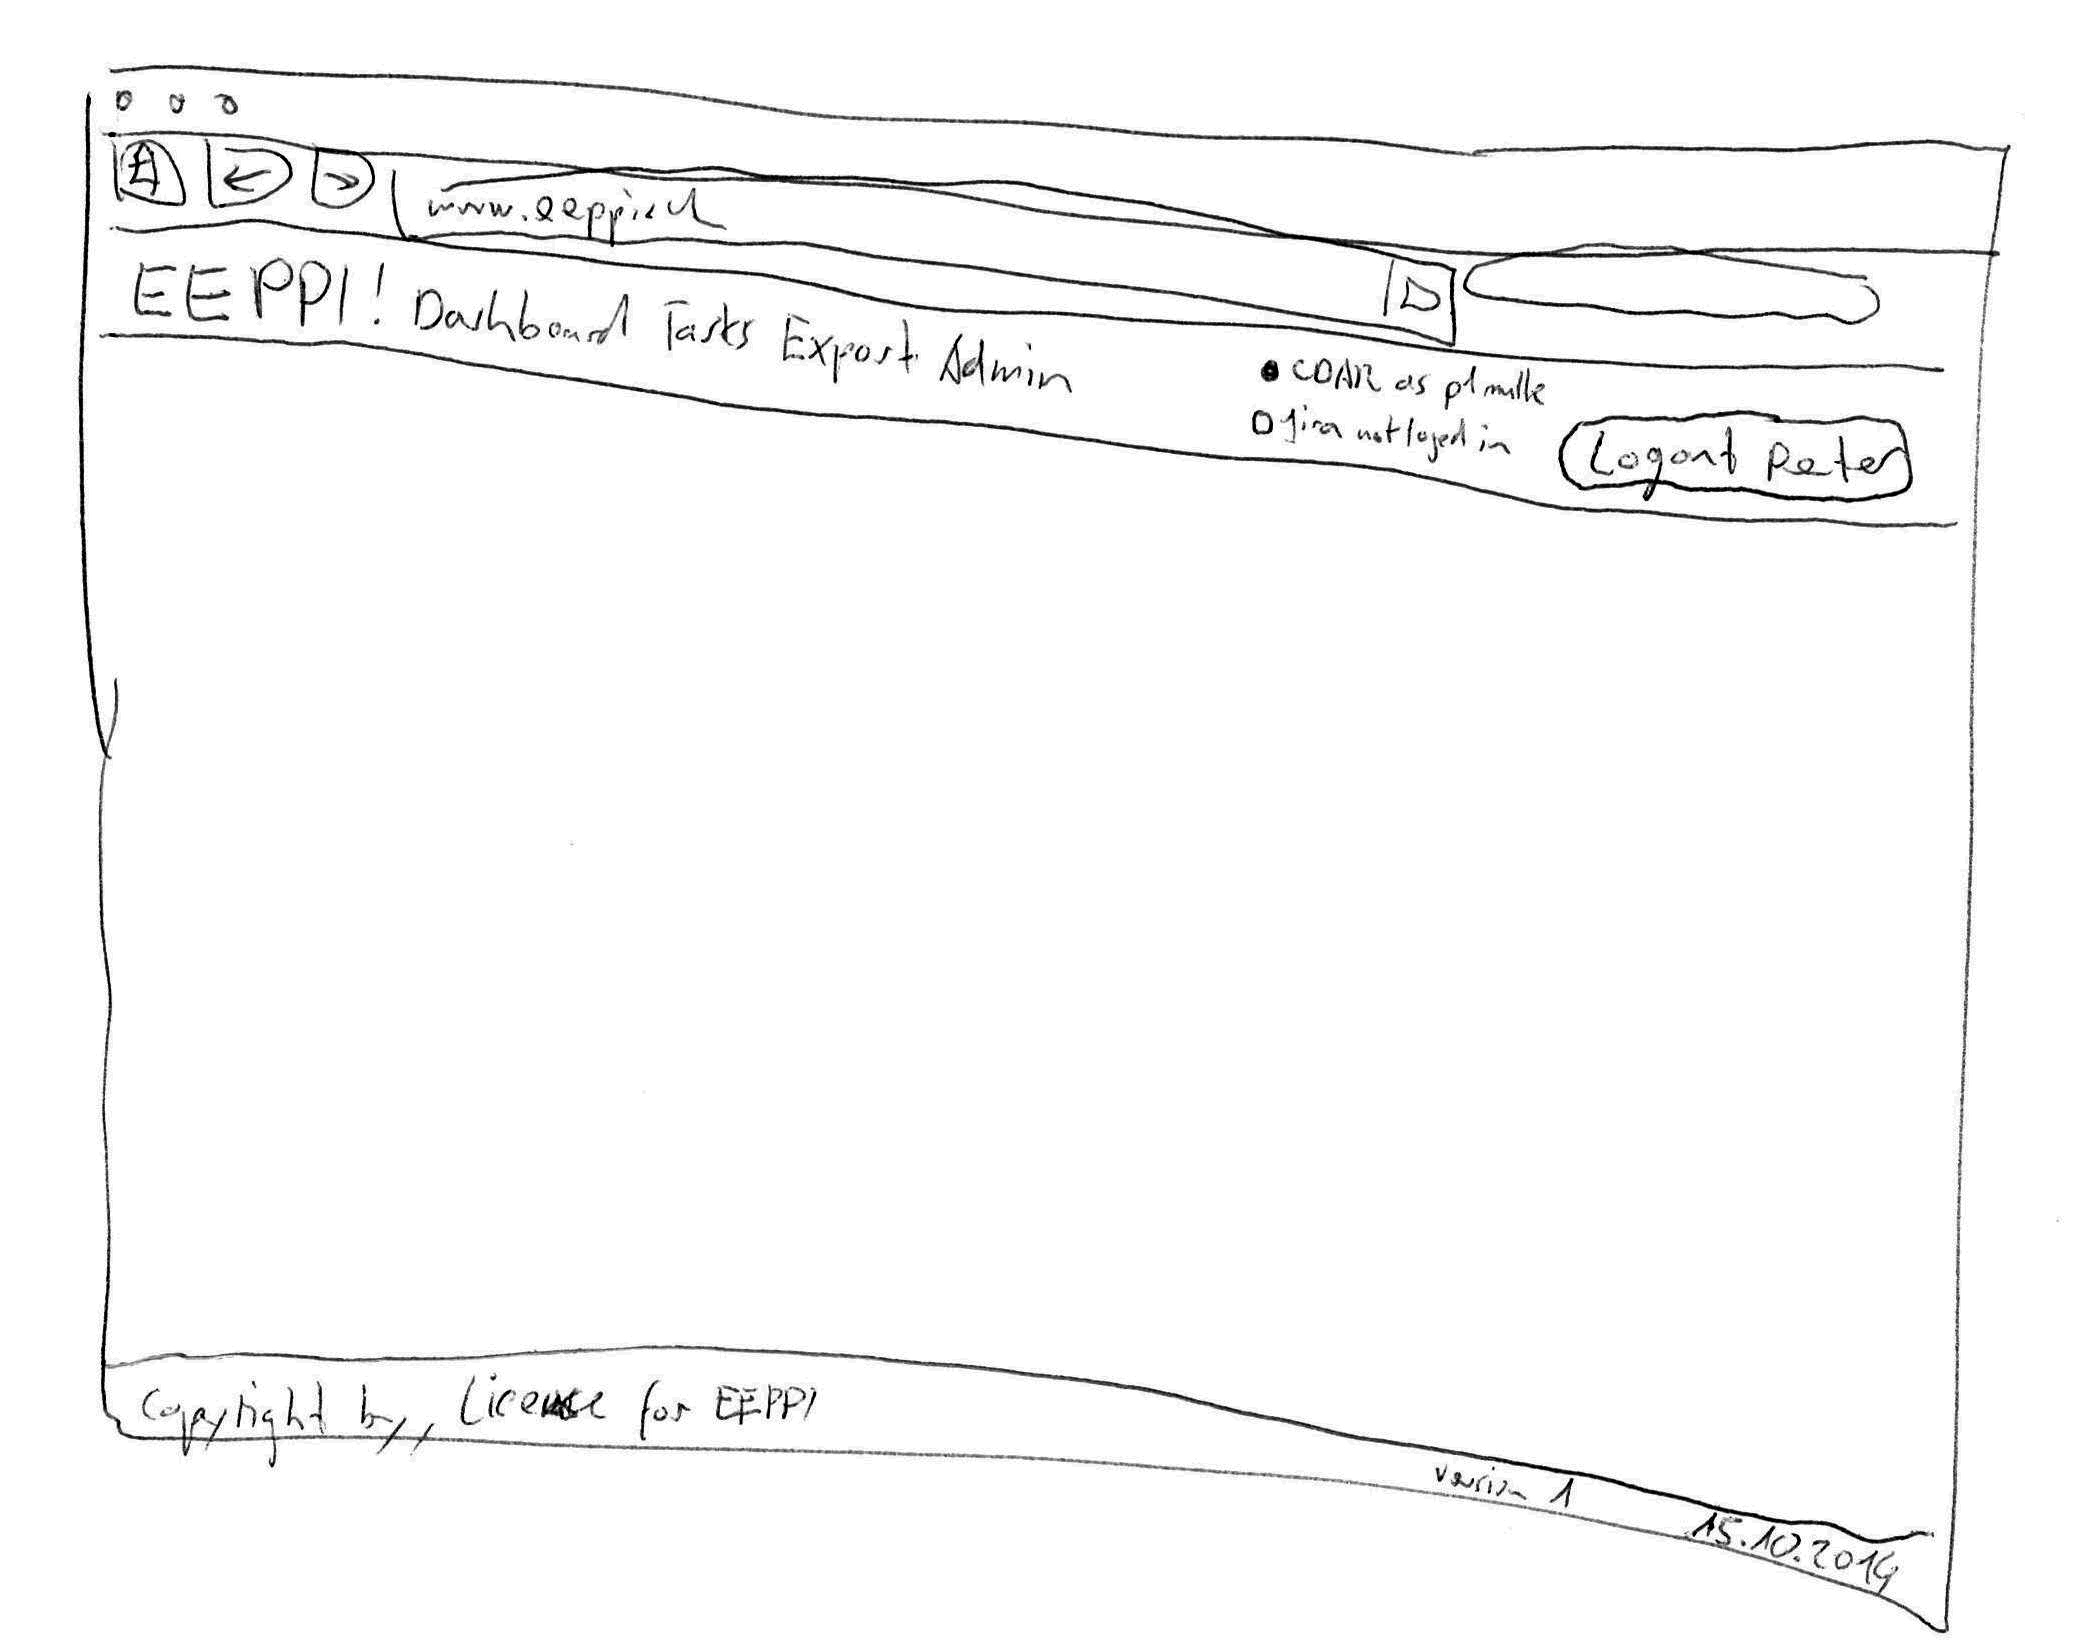
\includegraphics[width=\linewidth]{interfacesAndProtocols/media/img/wireframesLaurin1.jpg}
		\end{minipage}
		\begin{minipage}[b]{0.5\linewidth}	
			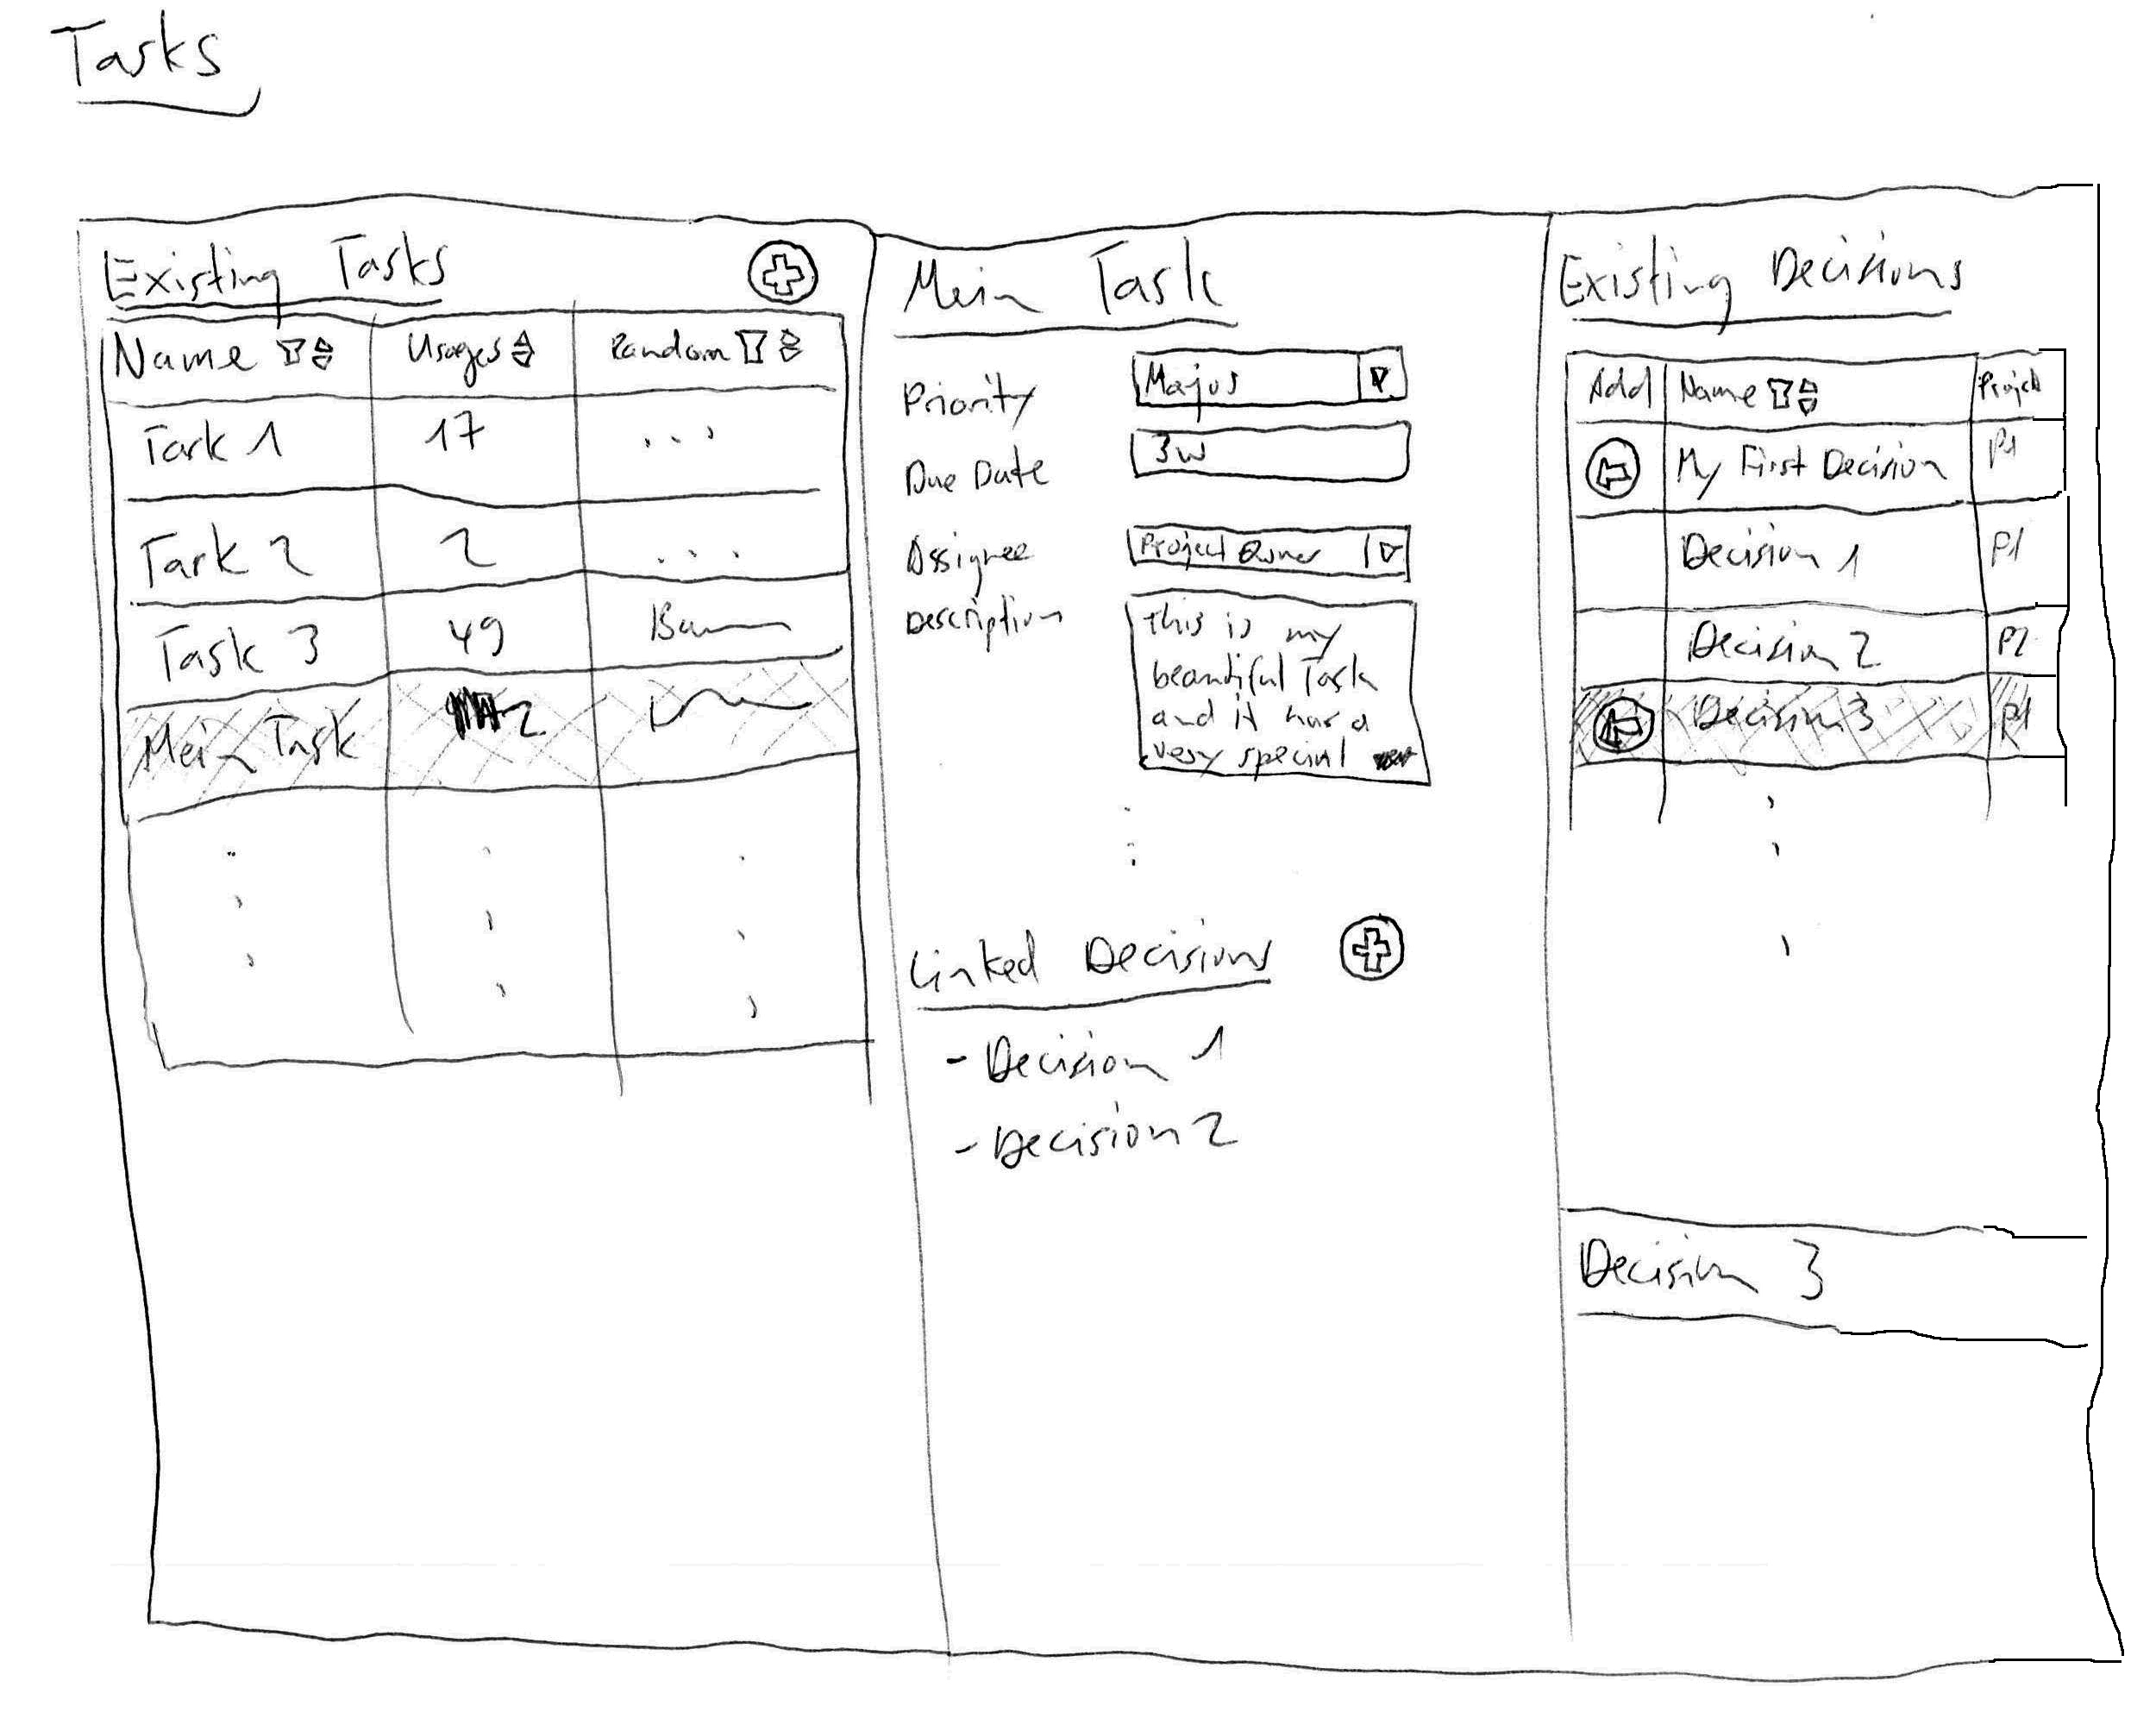
\includegraphics[width=\linewidth]{interfacesAndProtocols/media/img/wireframesLaurin2.jpg}
		\end{minipage}
	\end{figure}
	
	\begin{figure}[H]
		\begin{minipage}[b]{\linewidth}		
			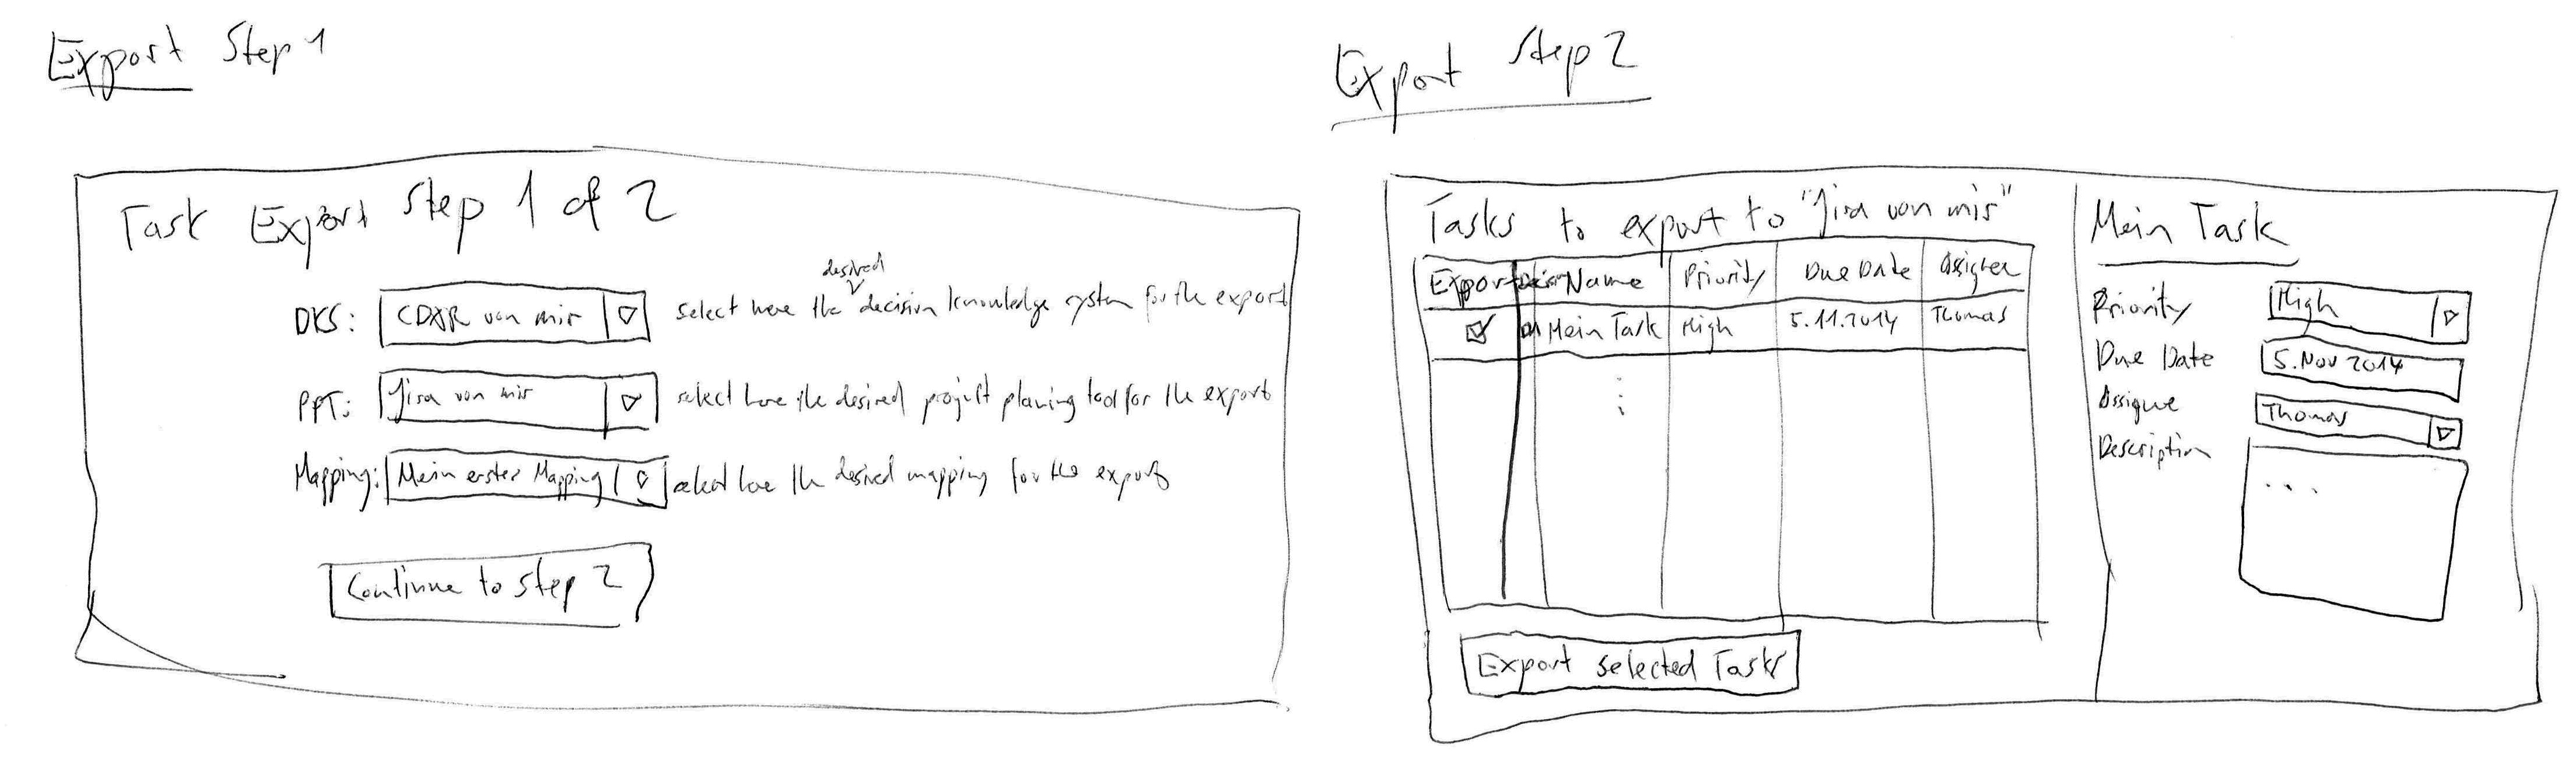
\includegraphics[width=\linewidth]{interfacesAndProtocols/media/img/wireframesLaurin3.jpg}
		\end{minipage}			
		\centering
		\caption{Wireframes Laurin}
		\label{fig:wireframesLaurin}
	\end{figure}
	
	Anschliessend wurden diese Entwürfe gemeinsam gesichtet, 
	Wireframes aussortiert oder ausgewählt und Ideen zu neuen Wireframes kombiniert.
	
	\begin{figure}[H]
		\begin{minipage}[b]{0.5\linewidth}
			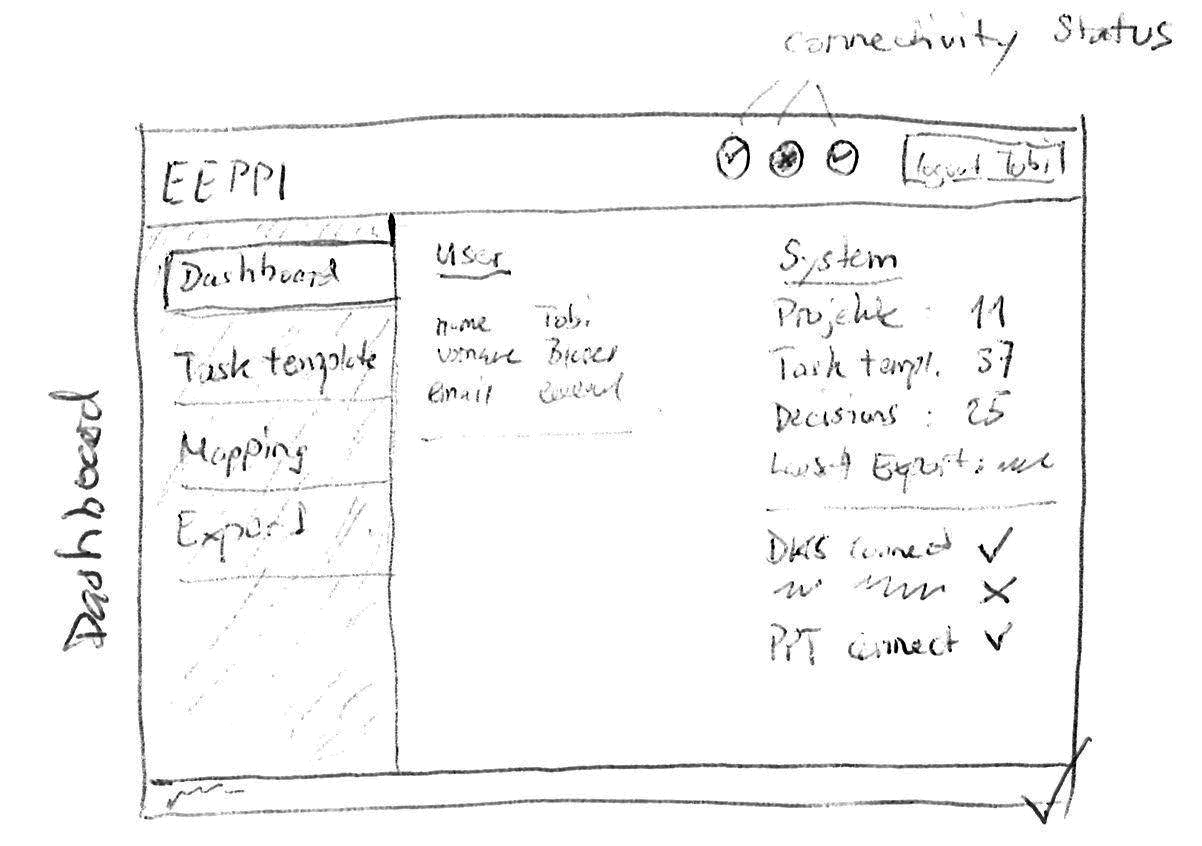
\includegraphics[width=\linewidth]{interfacesAndProtocols/media/img/dashboard.jpg}
		\end{minipage}
		\begin{minipage}[b]{0.5\linewidth}	
			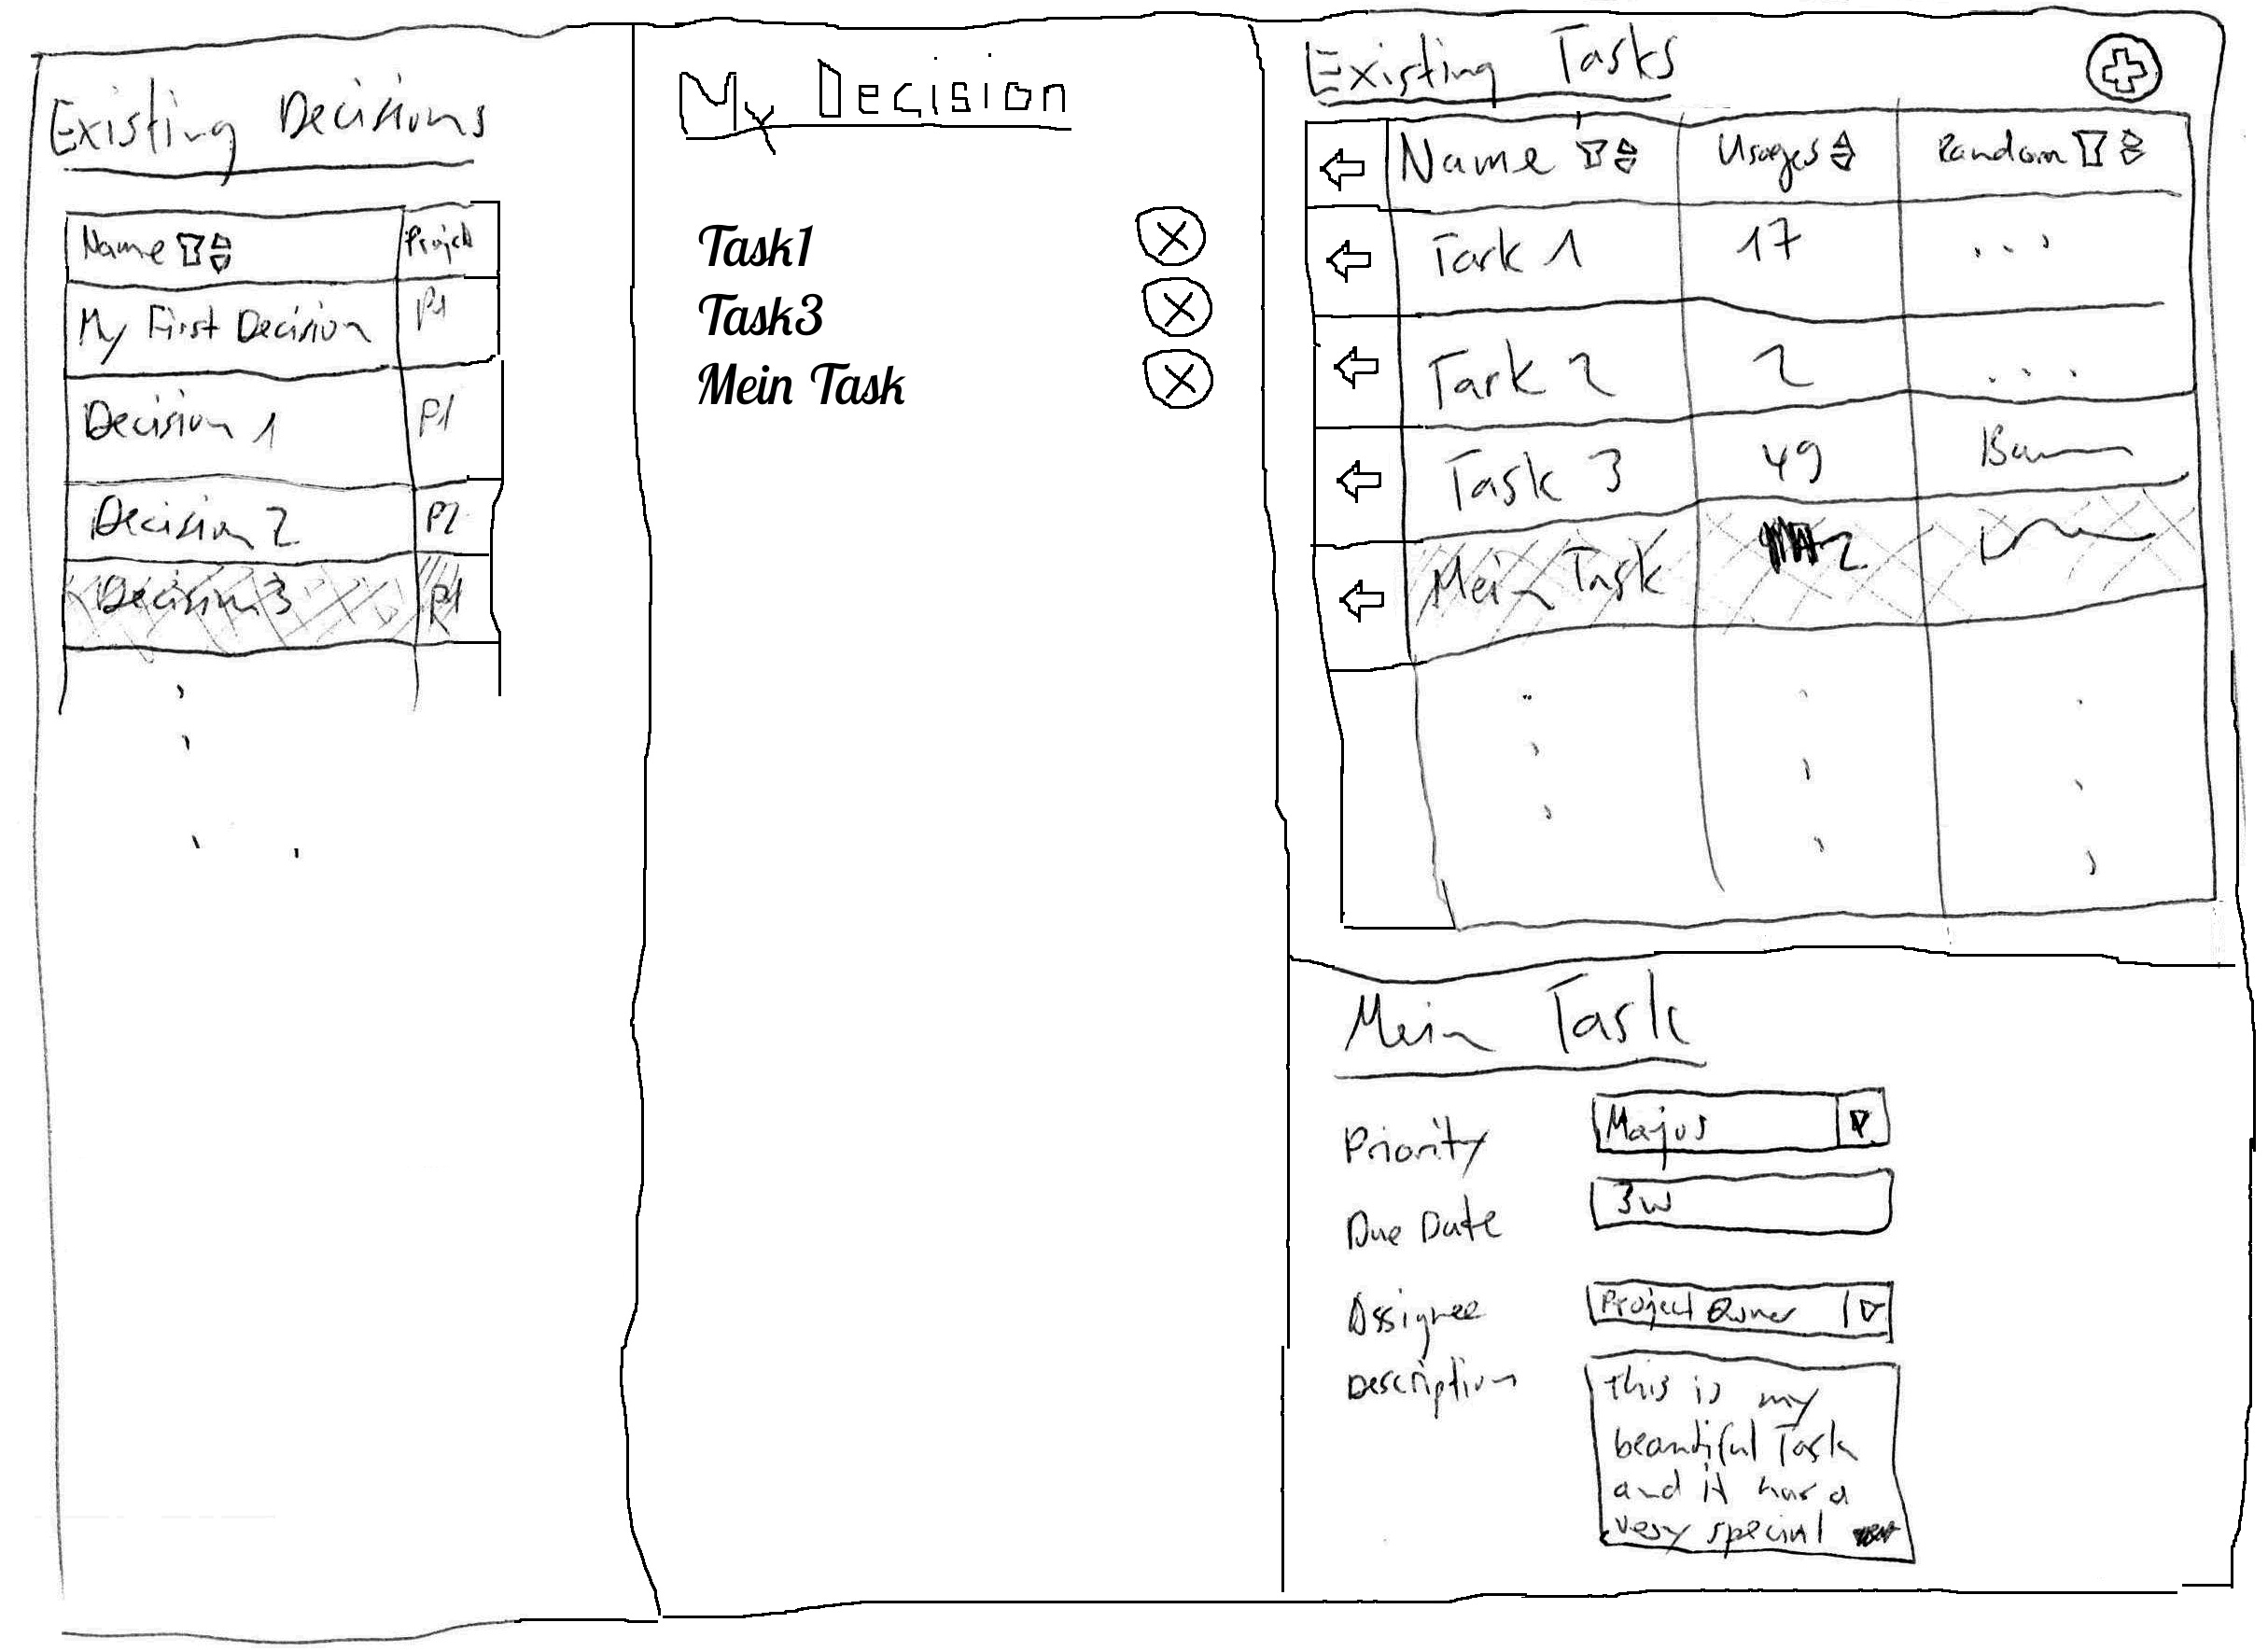
\includegraphics[width=\linewidth]{interfacesAndProtocols/media/img/tasks.jpg}
		\end{minipage}
		\caption{Dashboard \& Tasks}
		\label{fig:dashboardAndTasks}
	\end{figure}
	
	Für den Taskexport fiel die Entscheidung auf einen Assistent mit drei Schritten:
	\begin{enumerate}
		\item Auswählen von Projekt und DKS sowie des Mapping sets
		\item Bearbeiten der zu exportierenden Tasks, entfernen von nicht gewünschten
		\item Auswahl des PPT, exportieren sowie Übersicht über den Status eines laufenden Exports
	\end{enumerate}
	
	Eine Progressbar im unteren Bereich soll dem Benutzer jederzeit anzeigen, bei welchem Schritt er sich befindet.
	
	\begin{figure}[H]
		\begin{minipage}[b]{0.32\linewidth}
			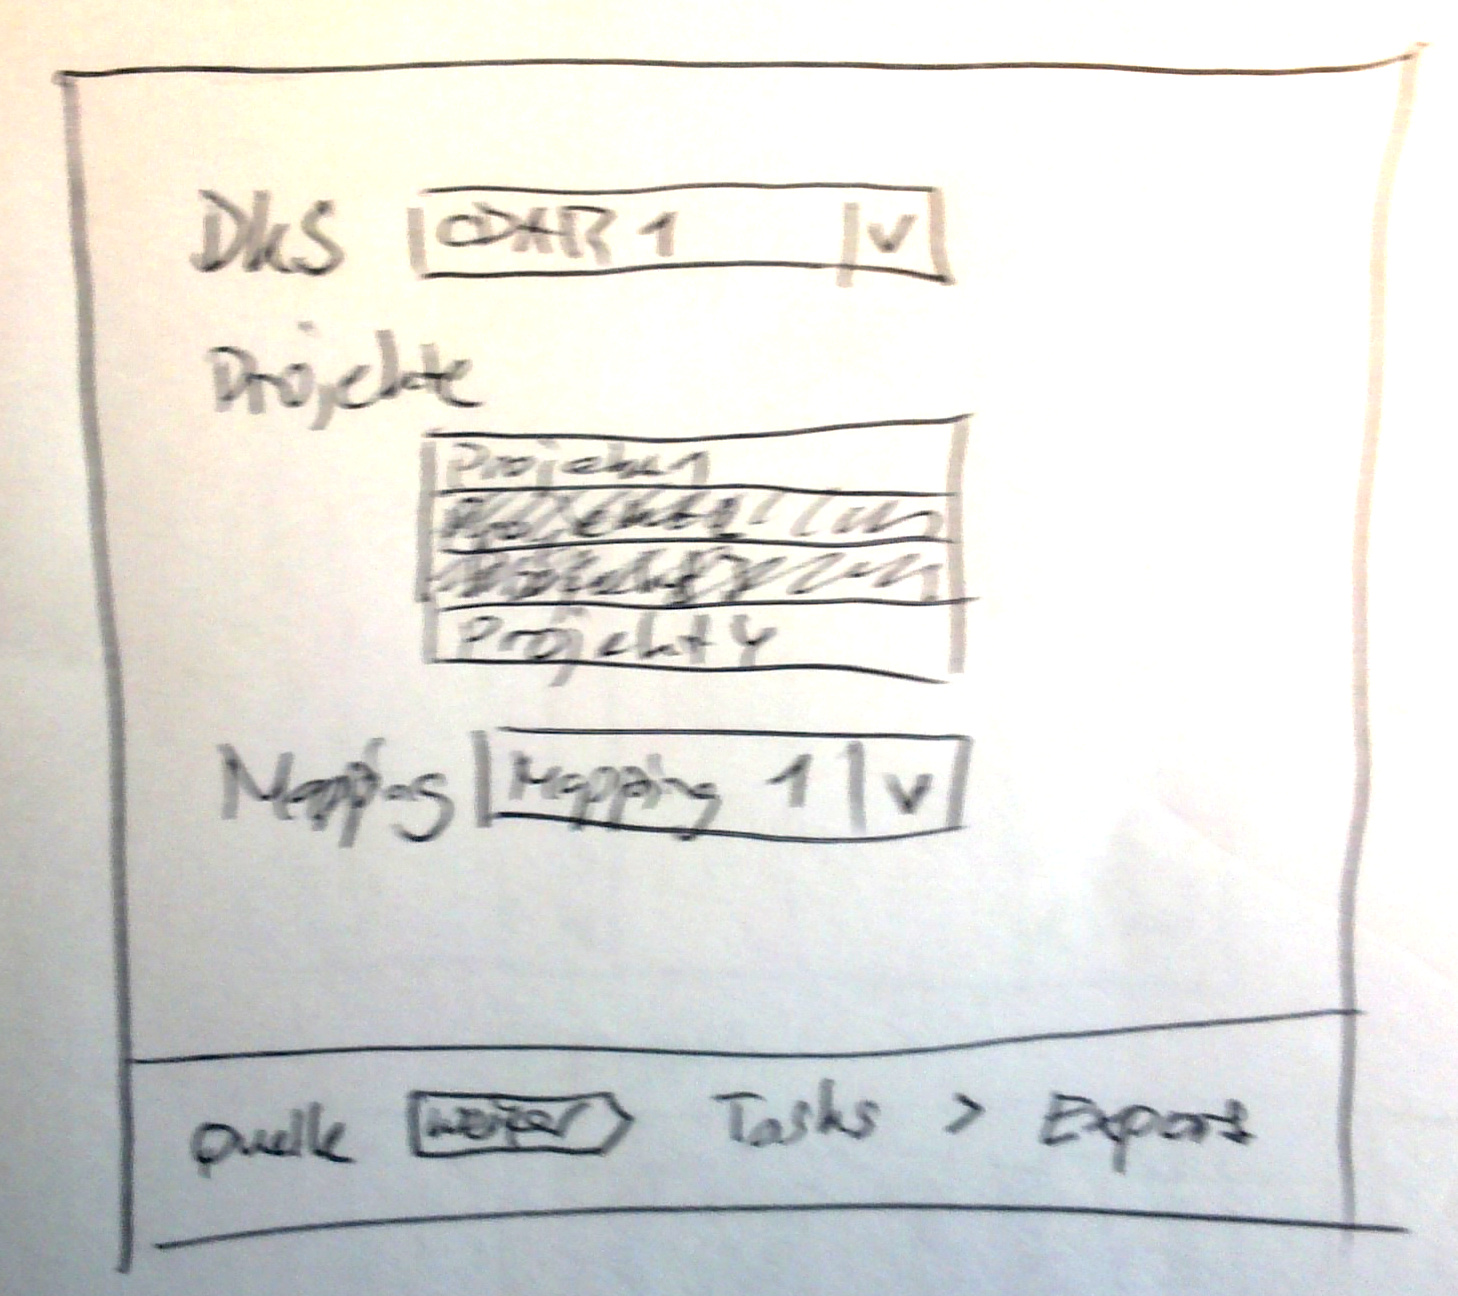
\includegraphics[width=\linewidth]{interfacesAndProtocols/media/img/export1.jpg}
		\end{minipage}
		\begin{minipage}[b]{0.30\linewidth}
			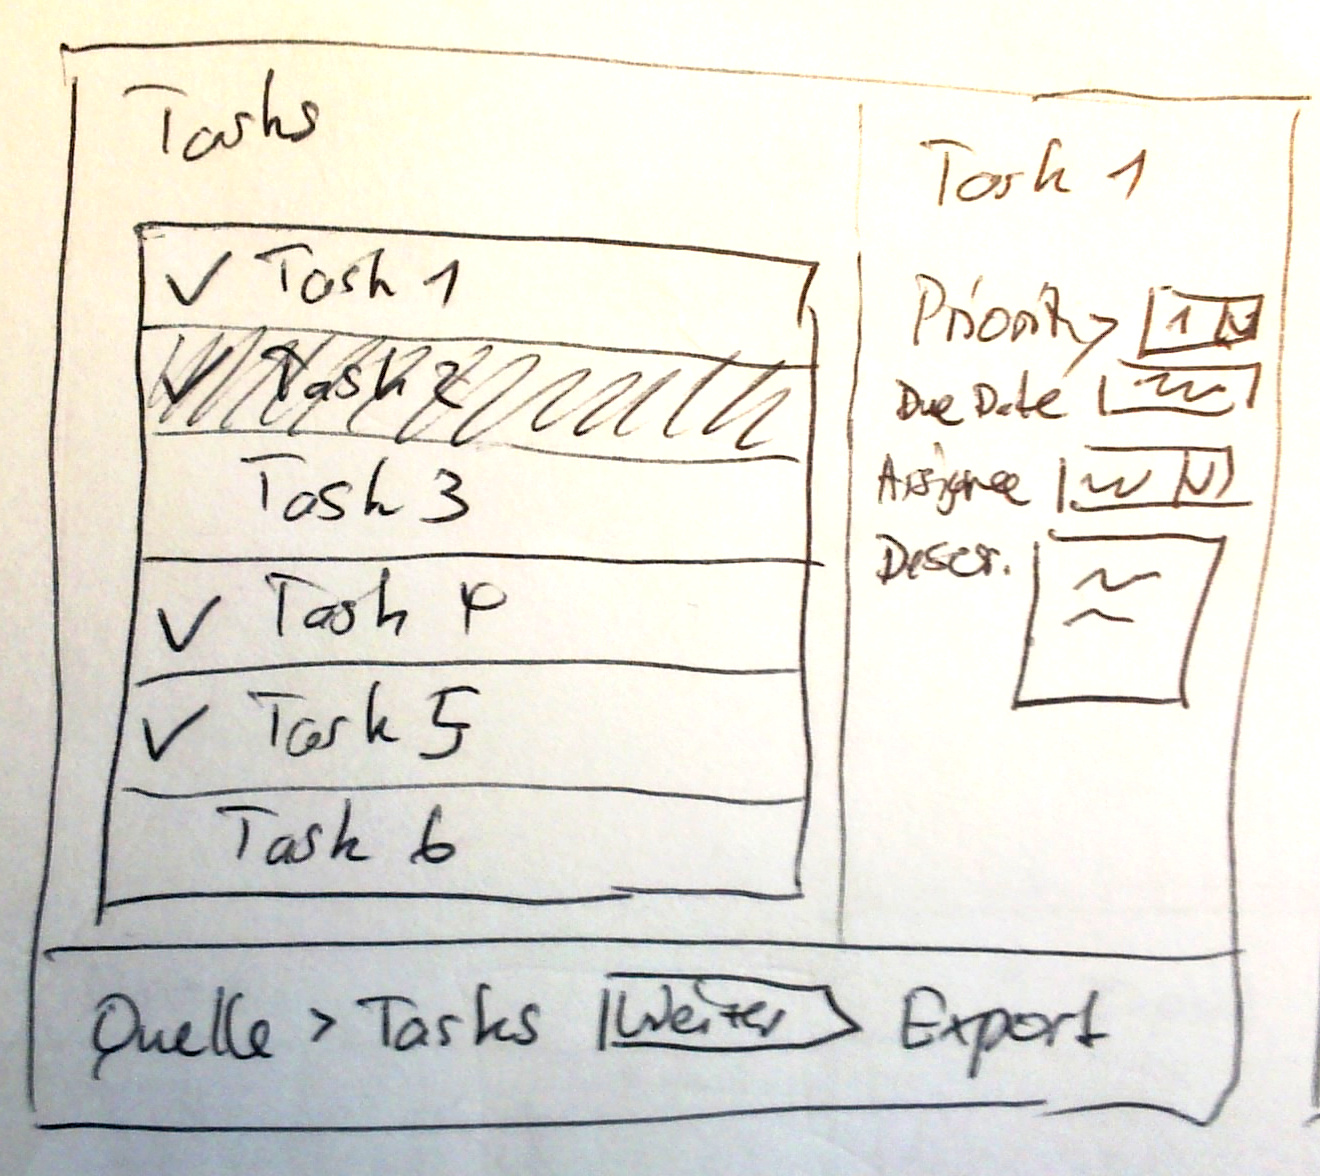
\includegraphics[width=\linewidth]{interfacesAndProtocols/media/img/export2.jpg}
		\end{minipage}
		\begin{minipage}[b]{0.34\linewidth}
			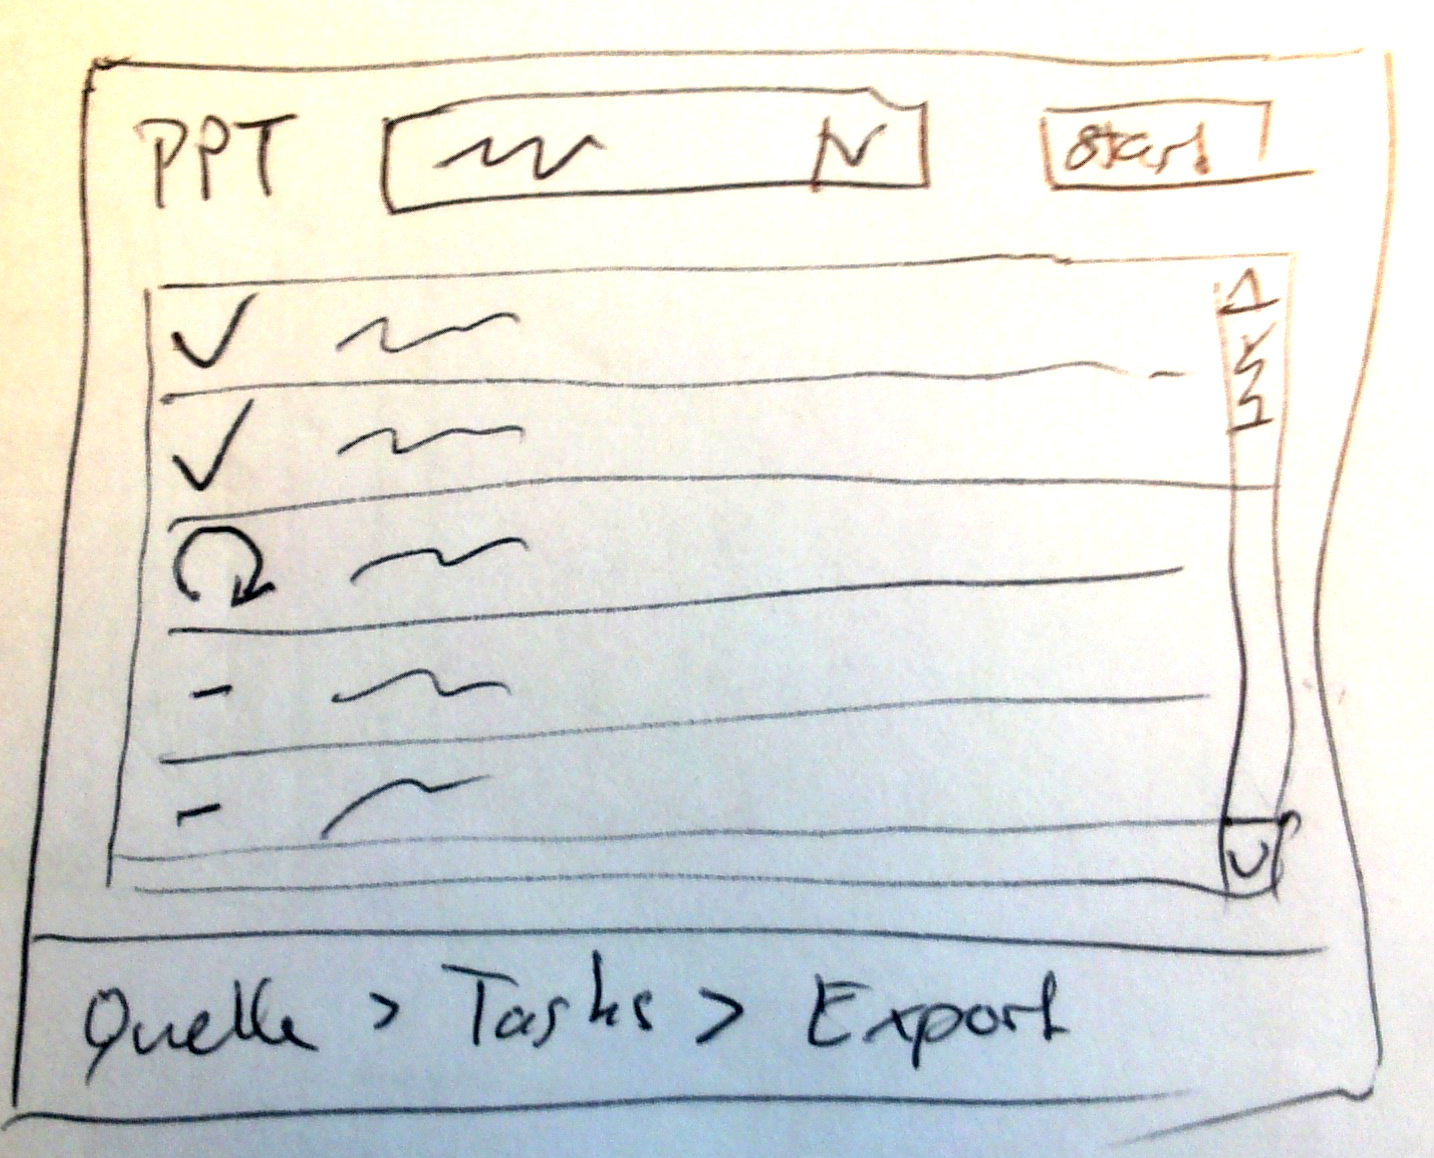
\includegraphics[width=\linewidth]{interfacesAndProtocols/media/img/export3.jpg}
		\end{minipage}
		\caption{Export Assistent}
		\label{fig:exportAssistent}
	\end{figure}	
	
	Der Benutzer kann nur weitergehen, nicht jedoch zurück, da dies durch den Umstand, 
	das aus Task-Vorlagen Tasks generiert werden, 
	zu Datenverlust führen könnte.